\documentclass[10pt]{article}
\usepackage{fullpage,amsfonts,mathpazo}
\usepackage{kotex}
\usepackage{mathtools}
\usepackage{tcolorbox}
\usepackage{caption}
\usepackage{subcaption}
\usepackage{graphicx}
\captionsetup[figure]{labelformat=empty}

\pagestyle{empty}

\begin{document}
\section*{AEA0165: Midterm (Due to: 2023/10/31 12:00, 연장미허용)}

\begin{enumerate}
	\item (20점) 아래 그림과 같이 주어진 단순지지보에 대해 다음 물음에 답하시오. 단 단면은 H-500$\times$200$\times$10$\times$16 (SS275)이고, $E=210,000\,\mathrm{MPa}$이다. 
	\begin{enumerate}
		\item 주어진 단면의 중립축으로부터의 단면2차모멘트를 구하시오. 
		\item 최대모멘트와 최대전단력을 구하시오. 
		\item 최대휨응력과 최대전단응력을 구하시오. 
		\item 최대휨응력으로부터 이 구조물의 안전여부를 판단하시오. 
	\end{enumerate}
	\vspace{-.2cm}
\begin{center}
	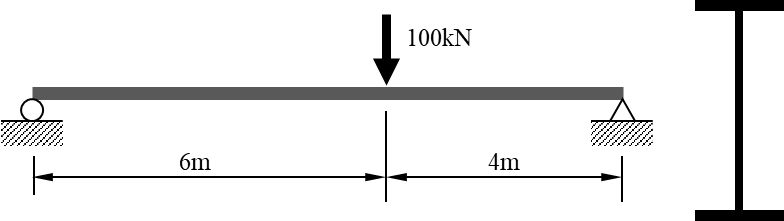
\includegraphics[scale=.7]{Mid202301}
\end{center}

	\item (20점) 아래 그림과 같이 주어진 단순지지보에 대해 다음 물음에 답하시오. 단 압축강도는 $27~\mathrm{MPa}$이고 $E=30,000\,\mathrm{MPa}$이다. 
	\begin{enumerate}
	\item 주어진 단면의 중립축으로부터의 단면2차모멘트를 구하시오. 
	\item 최대모멘트와 최대전단력을 구하시오. 
	\item 최대휨응력과 단부 $A$지점에서의 전단응력을 구하시오. 
	\item 최대휨응력으로부터 이 구조물의 안전여부를 판단하시오. 
\end{enumerate}
	\vspace{-.2cm}
\begin{center}
	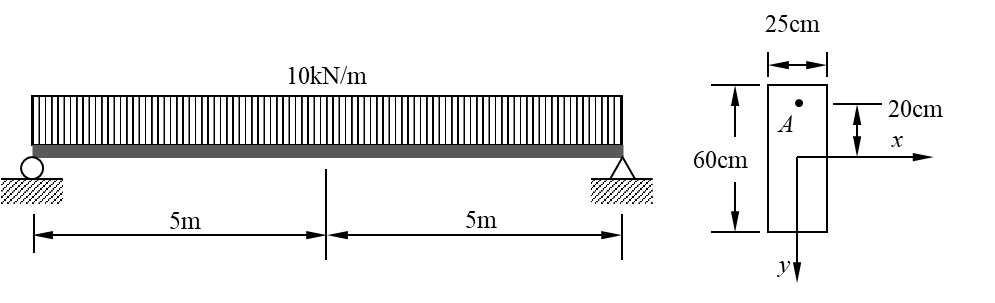
\includegraphics[scale=.7]{Mid202302}
\end{center}

	\item (20점) 아래 그림과 같이 주어진 캔틸레버보에 대해 다음 물음에 답하시오. 단 단면은 H-500$\times$200$\times$10$\times$16 (SS275)이고, $E=210,000\,\mathrm{MPa}$이다. 
	\begin{enumerate}
	\item 주어진 단면의 중립축으로부터의 단면2차모멘트를 구하시오. 
	\item 최대모멘트와 최대휨응력을 구하시오. 
	\item 최대응력이 나타나는 지점과 그 값을 구하시오.
	\item 최대응력으로부터 이 구조물의 안전여부를 판단하시오. 
\end{enumerate}
	\vspace{-.2cm}
\begin{center}
	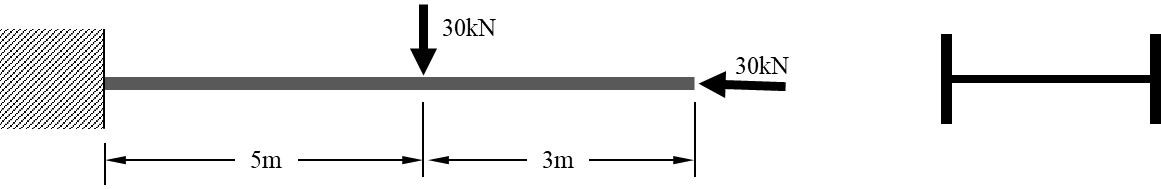
\includegraphics[scale=.7]{Mid202303}
\end{center}

%	\newpage
%	\item (20점) 아래 그림과 같이 주어진 단면에 대해 1) $x$-$y$축, 2) $X$-$Y$축과 3) 직각지점으로부터 회전된 $X'$축이 단면의 도심을 지나게 되는 $X'$-$Y'$축에 대한 단면2차모멘트와 단면상승모멘트를 구하시오(필요한 경우 교과서에 나온 값을 그대로 써도 상관없음).
%	\begin{figure}[h!]
%		\centering
%		\includegraphics[scale=.75]{Fig04.pdf} 
%	\end{figure}
%	\item (20점) 아래 그림과 같이 주어진 갤버보에서 최대휨응력과 최대전단응력이 발생하는 지점(또는 구간)을 구하고, 그 값들을 구하시오.
%	\begin{figure}[h]
%		\centering
%		\includegraphics[scale=.75]{Fig05.pdf} 
%	\end{figure}
\end{enumerate}
\end{document}
